\tikzstyle{compartment}=[circle, draw, thick, inner sep=0pt, minimum size=7mm]
\tikzstyle{pointto}=[->,shorten >=1pt,>=stealth,semithick]
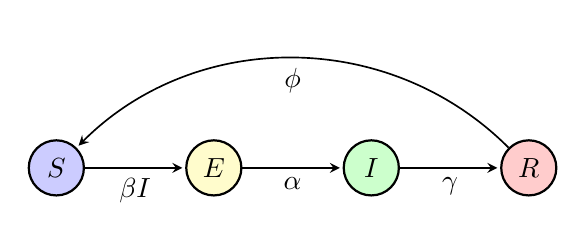
\begin{tikzpicture}
\node[compartment, fill=blue!20]  (S) at (0,0) {$S$};  % inner sep=6pt, 
\node[compartment, fill=yellow!20](E) at (2,0) {$E$};  % inner sep=6pt, 
\node[compartment, fill=green!20] (I) at (4,0) {$I$};  % inner sep=6pt, 
\node[compartment, fill=red!20]   (R) at (6,0) {$R$};  % inner sep=6pt, 
% \node[compartment](Q) at (4,-1) {Q}; % inner sep=6pt, 
\draw[pointto] (S) to node[below] {$\beta I$} (E);
\draw[pointto] (E) to node[below] {$\alpha$} (I);
\draw[pointto] (I) to node[below] {$\gamma$} (R);
\draw[pointto] (R) to[out=135, in=45] node[below] {$\phi$} (S);
\end{tikzpicture}
